\documentclass{jsarticle}
\usepackage{bm}
\usepackage[dvipdfmx]{graphicx}
\usepackage{amsthm}
\usepackage{amsmath,amssymb}
\usepackage{array,booktabs}
\usepackage{ascmac}
\usepackage{enumitem}
\usepackage{overcite}
\usepackage{listings}
\usepackage{plistings}
\usepackage{multicol}
\usepackage{url}

\newtheorem{dfn}{定義}[section]
\newtheorem{thm}[dfn]{定理}
\newtheorem{lem}[dfn]{補題}
\newtheorem{prop}[dfn]{命題}

\renewcommand{\proofname}{\bfseries 証明}
\newcommand{\relmiddle}[1]{\mathrel{}\middle#1\mathrel{}}

\lstset{language=C,frame=single, stepnumber=1,numbersep=5pt,tabsize=4,%
basicstyle=\footnotesize \ttfamily, stringstyle=\small\texttt, commentstyle=\slshape, captionpos=b,%
columns=[l]{fullflexible}}


\begin{document}
\title{所得格差指数の比の検定と検出力分析}
\author{奥城健太郎}
\date{2018年2月22日}
\maketitle
\thispagestyle{empty}

\newpage
\tableofcontents

%式ラベル : 13
%定理ラベル : 5

%%%%%%%%%%%%%%%%%%%%%%%%%%%%%%%%%%%%%%%%%%%%%%%%%%%%%%%%%%%%%%%%%%%%%%%%%%%%%%%%%%%%

\newpage
\section{はじめに}
筆者は,卒業研究として統計学について学習した.その中でも興味を持ったのは,確率分布を利用して注目している現象がどのような仮説に従っているかを判定する仮説検定や,その精度を高めるために必要なサンプル数を調べる検出力分析であった.本論文では,その応用例として所得格差指数の比の検定を行う.所得の分布は対数正規分布で近似できることが知られており,その対数正規分布のパラメータを用いて所得格差指数である\textbf{ジニ係数}を表すことができる.このジニ係数を求めるには集団内すべての人の所得が分かっていなければならない.しかし,統計学の理論を利用すればランダムに選んだ標本から母集団のジニ係数を推定することができる.本論文では,2つの集団から標本を採ってジニ係数を推定し,それらを比較する手法を提案する.この研究の目的は,ジニ係数が異なると判定できるのに必要なサンプル数を仮説検定の検出力分析を用いて明らかにすることである.

母集団が正規分布の場合の不偏分散推定量の存在はよく知られている.しかし,ジニ係数の不偏推定が可能かどうかの研究は見つけられなかった.そこで本論文では,\ref{test,power}章から\ref{syotoku}章で,統計学の教科書\cite{stat,size} やレポート\cite{geho,yosida} を参考に,$F$検定,ジニ係数,対数正規分布などについてまとめ,本論としては次の2点を述べる.まず,\ref{suitei}章でジニ係数の不偏推定が可能であることを示す.その後\ref{kentei}章で,推定したジニ係数の比をとり,それが$F$分布に従っているとして仮説検定を行う.しかし,推定ジニ係数の分布と$F$分布の間には誤差が存在するため,それを考慮した上でサンプル数を求める.

%%%%%%%%%%%%%%%%%%%%%%%%%%%%%%%%%%%%%%%%%%%%%%%%%%%%%%%%%%%%%%%%%%%%%%%%%%%%%%%%%%%%

\section{$F$検定と検出力}\label{test,power}
ジニ係数の比を検定するにあたって,2つの正規分布の分散比を検定する$F$検定を利用する.ここでは$F$検定の手順とそのサンプルサイズの設計方法について説明する.

\subsection{準備}
\begin{dfn}
次の確率密度関数を持つ確率分布を\textbf{正規分布}と呼び,$N(\mu, \sigma^2)$と表示する:
\[ f(x\mid \mu, \sigma^2)=\frac{1}{\sqrt{2\pi}\sigma}\exp \left\{ -\frac{(x-\mu)^2}{2\sigma^2}\right\} \ \ \  (-\infty<x<\infty).\]
また,正規分布の累積分布関数を$N(x\mid \mu, \sigma^2)$とする.すなわち,
\[ N(x\mid \mu, \sigma^2)=\int_{-\infty}^x \frac{1}{\sqrt{2\pi}\sigma}\exp \left\{ -\frac{(u-\mu)^2}{2\sigma^2} \right\} du \]
となる.
\end{dfn}

\begin{dfn}
$u_1,u_2,\dotsb ,u_k\sim N(0,1)$で,互いに独立のとき,
\[ \chi^2=u_1^2+u_2^2+\dotsb+u_k^2=\sum_{i=1}^k u_i^2 \]
の確率分布を自由度$\phi=k$の\textbf{$\chi^2$分布}と呼び,$\chi^2(\phi)$と表示する.\\
ここで,“$X\sim F(\cdot)$”とは「確率変数$X$は分布$F(\cdot)$に従う」という意味である.
\end{dfn}

\begin{dfn}
$ \chi_1^2 \sim \chi ^2 (\phi_1) , \chi_2^2 \sim \chi ^2 (\phi_2) $ で,互いに独立のとき,
\[ F=\frac{ \chi_1^2 / \phi_1 }{ \chi_2^2 / \phi_2 } \]
の確率分布を自由度 ($\phi_1,\phi_2$) の\textbf{$F$分布}と呼び,$F(\phi_1,\phi_2)$と表示する.
\end{dfn}

\ \\
次の定理\ref{t3}と定理\ref{t4}は正規分布の分散の比の検定で用いるものである.

\begin{thm} \label{t3}
$ x_{11}, x_{12}, \dotsb, x_{1n_1} \sim N(\mu_1, \sigma_1^2),\  x_{21}, x_{22}, \dotsb, x_{2n_2} \sim N(\mu_2, \sigma_2^2) $
で,すべて互いに独立とする.
$ V_1 = \sum_{i=1}^{n_1} (x_{1i}-\overline{x}_1)^2/(n_1-1) $,$ V_2 = \sum_{i=1}^{n_2} (x_{2i}-\overline{x}_2)^2/(n_2-1) $
とする.($V_1,V_2$を不偏分散という.)\\
このとき次が成り立つ:
\[ \frac{V_1/\sigma_1^2}{V_2/\sigma_2^2} \sim F(n_1-1,n_2-1). \]
\end{thm}

\begin{thm}[コーニッシュ・フィッシャーの近似式] \label{t4}
$ F \sim F(\phi,\phi) $のとき,$ \dfrac{1}{2} \ln F $ は近似的に $ N(0,1/\phi) $ に従う.
\end{thm}


\subsection{統計的仮説検定と検出力分析}
\subsubsection{統計的仮説検定}
統計的仮説検定はある事象がどのような仮説のもとで成り立っているのかを推定する方法であり,次のような手順で行われる.
\begin{enumerate}
\item 中心となる仮説(\textbf{帰無仮説})とそれに相対する仮説(\textbf{対立仮説})を用意する.
\item 検証したい事象に対して,帰無仮説が正しいとしたときにその事象またはそれより起こりにくい事象が起こる確率(\textbf{$p$値})を求める.
\item $p$値がある一定の値(\textbf{有意水準})より大きければ帰無仮説を採択,小さければ帰無仮説を棄却して対立仮説を採択する.
\end{enumerate}
統計的仮説検定を略して仮説検定,検定ともいう.

\subsubsection{2種類の誤りと検出力分析}
帰無仮説が正しいのに帰無仮説を棄却してしまうことを\textbf{第1種の誤り}といい,帰無仮説が誤っているのに帰無仮説を採択してしまうことを\textbf{第2種の誤り}という.第1種の誤りが起こる確率を$\alpha$,第2種の誤りが起こる確率を$\beta$で表し,特に$1-\beta$を検出力という.$\alpha$と$\beta$は一方を小さくするともう一方が大きくなる関係にあるため,$\alpha$を一定に保った上で$\beta$を小さくすることを考える.$\beta$を小さくするにはサンプル数を大きくしたり,帰無仮説と対立仮説の差を大きくしたりすればよい.サンプル数や仮説間の差を変化させて検出力$1-\beta$がどのように変化するかを調べるのが\textbf{検出力分析}である.


\subsection{2つの正規分布の分散比の検定} \label{ftest}
$F$分布の性質を用いて,2つの正規分布する集団の母分散の比を検定することができる.この検定を\textbf{$F$検定 \ ($F$-test)}という.

\subsubsection{検定手順}
\begin{enumerate}[label=手順\arabic*]
\item 仮説の設定\\
2つの集団の母分散をそれぞれ$\sigma_1^2$,$\sigma_2^2$($\sigma_1\geq \sigma_2$)とする.
このとき,帰無仮説と対立仮説を次のように設定する:\\
帰無仮説 $ H_0 : \sigma_1^2 = \sigma_2^2 $ \\
対立仮説 $ H_1 : \sigma_1^2 > \sigma_2^2 $.
\item 有意水準$\alpha$の設定 (通常は$\alpha =0.05$とする)
\item データ $ x_{11}, x_{12}, \dotsb, x_{1n_1} $ および $ x_{21}, x_{22}, \dotsb, x_{2n_2} $ をとり,検定統計量$F_0$の値を計算する.
\begin{align*}
F_0 &=\frac{V_1}{V_2} \\
V_1 &=\frac{S_1}{n_1-1} = \frac{\sum_{i=1}^{n_1} (x_{1i}-\overline{x}_1)^2}{n_1-1} \\
&=\frac{\sum x_{1i}^{2} - (\sum x_{1i})^2/n_1}{n_1-1} \\
V_2 &=\frac{S_2}{n_2-1} = \frac{\sum_{i=1}^{n_2} (x_{2i}-\overline{x}_2)^2}{n_2-1} \\
&=\frac{\sum x_{2i}^{2} - (\sum x_{2i})^2/n_2}{n_2-1} \\
\phi_1 &=n_1-1 \\
\phi_2 &=n_2-1
\end{align*}
\item 棄却域$R$の設定
\[ R : F_0\geq F(\phi_1, \phi_2; \alpha) \]
\item $F_0$が手順4で設定した棄却域$R$にあれば有意と判定し,$H_0$を棄却する.
\end{enumerate}
\ \\
上の検定方式で,$F(\phi_1, \phi_2; P)$ は自由度$(\phi_1, \phi_2)$ の$F$分布の\textbf{上側} $100P\%$ \textbf{点},すなわち,
\begin{equation}
\mathrm{Pr}\{ F\geq F(\phi_1, \phi_2; P)\} =P \label{1}
\end{equation}
である.

\subsubsection{検出力の導出}
検出力$1-\beta$は$H_1 : \sigma_1^2>\sigma_2^2$の下で計算する.
$H_1$の下では$F=\dfrac{V_1/\sigma_1^2}{V_2/\sigma_2^2}$が自由度
$(\phi_1, \phi_2)=(n_1-1, n_2-1)$の$F$分布に従うので,$\Delta=\sigma_1/\sigma_2$とすると,検出力$1-\beta$は
\begin{align}
1-\beta &=\mathrm{Pr}\{F_0\geq F(\phi_1, \phi_2; \alpha)\} \notag \\
&=\mathrm{Pr}\left\{ \frac{V_1}{V_2}\geq F(\phi_1, \phi_2; \alpha)\right\} \notag \\
&=\mathrm{Pr}\left\{ \frac{V_1/\sigma_1^2}{V_2/\sigma_2^2}\times \frac{\sigma_1^2}{\sigma_2^2}\geq F(\phi_1, \phi_2; \alpha)\right\} \notag \\
&=\mathrm{Pr}\left\{ F\geq \frac{F(\phi_1, \phi_2; \alpha)}{\Delta^2}\right\} \label{2}
\end{align}
となる.

\subsubsection{サンプルサイズの設計}
$\Delta=\sigma_1/\sigma_2$について,$\Delta \geq \Delta_0$のとき高い検出力$1-\beta$で$H_0$を棄却したい.そのためのサンプルサイズ$n$の設計方法を考える.ここでは2つの標本のサンプルサイズが等しいとする.

$\phi_1=\phi_2=n-1=\phi$とおく.このとき,\eqref{1}より
\[ \mathrm{Pr}\{F\geq F(\phi, \phi; P)\}=P \]
である.これより,
\[ \mathrm{Pr}\left\{ \frac{1}{2}\log F\geq \frac{1}{2}\log F(\phi, \phi; P)\right\}=P \]
となる.$N(0,1)$に従う確率変数$u$に対して,上側$100P\%$点を$z_P$とすると,
\[ \mathrm{Pr}(u\geq z_P)=P \]
だから,コーニッシュ・フィッシャーの近似式に基づくと,$\dfrac{\sqrt{\phi}}{2}\log F\approx u$なので,
\[ \frac{\sqrt{\phi}}{2}\log F(\phi, \phi; P)\approx z_P \]
と考えることができる.したがって,次式が成り立つ.
\begin{equation}
F(\phi, \phi; P)\approx \exp \left(\frac{2z_P}{\sqrt{\phi}}\right) \label{3}
\end{equation}
よって,\eqref{2},\eqref{3}より,
\begin{align}
1-\beta &=\mathrm{Pr}\left\{ F\geq \frac{F(\phi, \phi; \alpha)}{\Delta_0^2}\right\} \notag \\
&\approx \mathrm{Pr}\left\{F\geq \frac{1}{\Delta_0^2}\exp \left(\frac{2z_{\alpha}}{\sqrt{\phi}}\right) \right\} \label{4}
\end{align}
を得る.したがって,\eqref{3},\eqref{4}より,
\[ \frac{1}{\Delta_0^2}\exp \left(\frac{2z_{\alpha}}{\sqrt{\phi}}\right) \approx F(\phi, \phi; 1-\beta)
\approx \exp \left(\frac{2z_{1-\beta}}{\sqrt{\phi}}\right) \]
となる.これより,両辺の自然対数をとり,$\phi=n-1$であることに注意して$n$について解くと,
\[ n\approx 1+\left(\frac{z_{\alpha}-z_{1-\beta}}{\log \Delta_0}\right)^2 \]
が成り立つ.

%%%%%%%%%%%%%%%%%%%%%%%%%%%%%%%%%%%%%%%%%%%%%%%%%%%%%%%%%%%%%%%%%%%%%%%%%%%%%%%%%%%%%%%%%%%%

\section{順序統計量}
\begin{dfn}
累積分布関数$F(x)$と確率密度関数$f(x)$
同一の分布からの無作為標本$X_1,X_2,\dotsb,X_n$を大きさの順に並べたものを
\[ X_{n:1} \leq X_{n:2} \leq \dotsb X_{n:n} \]
と書き,\textbf{順序統計量}(order statistics)という.
\end{dfn}

\begin{prop}
累積分布関数が$F(x)$,確率密度関数が$f(x)$となるような分布に標本$X_1,X_2,\dotsb,X_n$が従っており,
$r$番目の順序統計量$X_{n:r}$の確率密度関数を$f_r(x)$とすると,
\begin{equation}
f_r(x)=r\binom{n}{r}F(x)^{r-1}\{1-F(x)\}^{n-r}f(x) \label{9}
\end{equation}
となる.
\end{prop}

\begin{proof}
まず,$X_{n:r}$の累積分布関数$F_r(x)$を求める.$X_{n:n+1}=\infty$とおく.次のような事象の同値性に着目する:
\[ \{X_{n:i}\leq x<X_{n:i+1}\} \Longleftrightarrow i=\# \{h\mid X_h\leq x\} \Longleftrightarrow n-i=\# \{h\mid X_h>x\} . \]
そこで,$x$以下のときを成功とみなし$x$を越えるときを失敗とみなせば,成功の確率が$p=\mathrm{Pr}(X\leq x)=F(x)$の二項確率となるので,
\[ \mathrm{Pr}(X_{n:i}\leq x<X_{n:i+1})=\binom{n}{i}F(x)^i\{1-F(x)\}^{n-i} \]
である.ゆえに,$F_r(x)$は
\begin{align*}
F_r(x) &=\mathrm{Pr}(X_{n:r}\leq x) \\
&=\sum_{i=r}^n \mathrm{Pr}(X_{n:i}\leq x<X_{n:i+1}) \\
&=\sum_{i=r}^n \binom{n}{i}F(x)^i\{1-F(x)\}^{n-i}.
\end{align*}
したがって,$f_r(x)$は
\begin{align*}
f_r(x)= &\frac{dF_r(x)}{dx} \\
=&\sum_{i=r}^n \binom{n}{i} [iF(x)^{i-1}\{1-F(x)\}^{n-i}f(x)-(n-i)F(x)^i\{1-F(x)\}^{n-i-1}f(x)] \\
=&\binom{n}{r} rf(x)F(x)^{r-1}\{1-F(x)\}^{n-r}+\sum_{i=r+1}^n \binom{n}{i} iF(x)^{i-1}\{1-F(x)\}^{n-i}f(x) \\
&-\sum_{i=r}^{n-1} \binom{n}{i} (n-i)F(x)^i\{1-F(x)\}^{n-i-1}f(x) \\
=&\binom{n}{r} rf(x)F(x)^{r-1}\{1-F(x)\}^{n-r}+\sum_{i=r}^{n-1} \binom{n}{i+1} (i+1)F(x)^i\{1-F(x)\}^{n-i-1}f(x) \\
&-\sum_{i=r}^{n-1} \binom{n}{i} (n-i)F(x)^i\{1-F(x)\}^{n-i-1}f(x) \\
=&r\binom{n}{r} F(x)^{r-1}\{1-F(x)\}^{n-r}f(x).
\end{align*}
\end{proof}

%%%%%%%%%%%%%%%%%%%%%%%%%%%%%%%%%%%%%%%%%%%%%%%%%%%%%%%%%%%%%%%%%%%%%%%%%%%%%%%%%%%%%%%%%%%%%%%%%%%%%%%%

\section{所得格差とは} \label{syotoku}
\subsection{所得の分布と対数正規分布の性質}
所得の分布は\textbf{対数正規分布}で近似できる.
\begin{dfn}
確率変数$Y=\log X$が正規分布$N(\mu, \sigma^2)$に従うとき,確率変数$X$が従う分布を\textbf{対数正規分布}と呼び,$\Lambda(\mu, \sigma^2)$と表示する.
\end{dfn}

\begin{figure}[htbp]
\centering
\begin{minipage}{0.52\columnwidth}
\centering
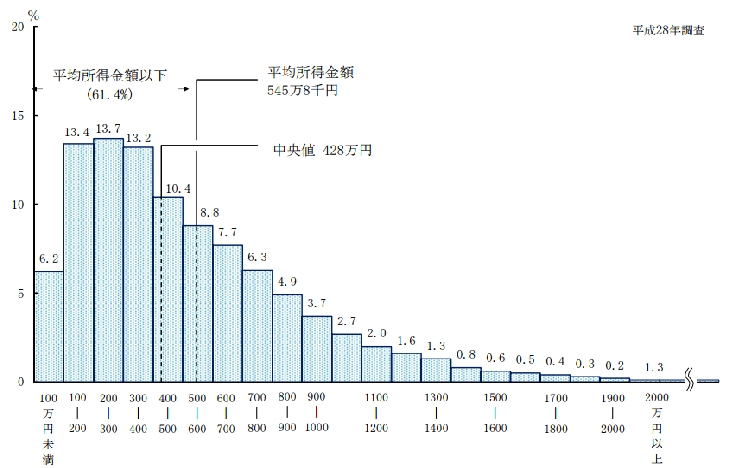
\includegraphics[width=\columnwidth]{figure2}
\caption{日本の所得分布 \cite{URL1}}
\end{minipage}
\begin{minipage}{0.47\columnwidth}
\centering
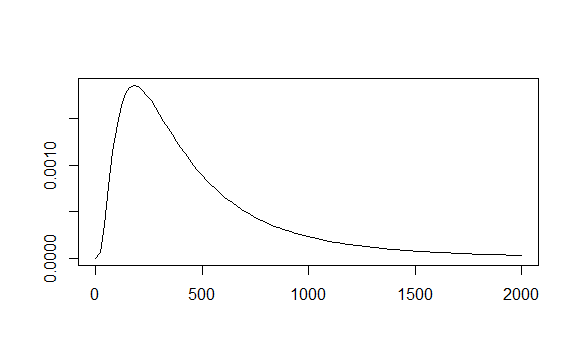
\includegraphics[width=\columnwidth]{figure3}
\caption{$\Lambda(5.9,0.7)$の確率密度関数 (平均:$555$)}
\end{minipage}
\end{figure}

\begin{prop}
対数正規分布の累積分布関数を$\Lambda(x\mid \mu, \sigma^2)$とすると,
\[ \Lambda(x\mid \mu, \sigma^2)=\int_0^x \frac{1}{\sqrt{2\pi}\sigma t}\exp \left\{ -\frac{(\log t-\mu)^2}{2\sigma^2}\right\} dt \]
となる.
\end{prop}

\begin{proof}
確率変数$Y$が正規分布$N(\mu, \sigma^2)$に従うとき,その累積分布関数$N(y\mid \mu, \sigma^2)$は,
\[ N(y\mid \mu, \sigma^2)=\int_{-\infty}^y \frac{1}{\sqrt{2\pi}\sigma}\exp \left\{ -\frac{(u-\mu)^2}{2\sigma^2}\right\} du \]
となる.このとき,確率変数$X$を$X=e^Y$とすると$X\sim \Lambda(\mu, \sigma^2)$となり,その累積分布関数$\Lambda(x\mid \mu, \sigma^2)$は$t=e^u$の変数変換により,
\begin{align*}
\Lambda(x\mid \mu, \sigma^2) &=\int_0^x \frac{1}{\sqrt{2\pi}\sigma}\exp \left\{ -\frac{(\log t-\mu)^2}{2\sigma^2}\right\} \frac{du}{dt}\ dt \\
&=\int_0^x \frac{1}{\sqrt{2\pi}\sigma t}\exp \left\{ -\frac{(\log t-\mu)^2}{2\sigma^2}\right\} dt
\end{align*}
となる.
\end{proof}

\newpage

\begin{prop}
対数正規分布$\Lambda(\mu, \sigma^2)$の期待値を$m$とすると,
\[ m=\exp \left( \mu+\frac{\sigma^2}{2}\right) \]
となる.
\end{prop}

\begin{proof}
\begin{align*}
m &=\int_0^{\infty}x\ d\Lambda(x\mid \mu, \sigma^2) \\
&=\int_{-\infty}^{\infty}e^y\ dN(y\mid \mu, \sigma^2) \hspace{1cm} \text{($x=e^y$と変数変換をした)} \\
&=\frac{1}{\sqrt{2\pi}\sigma}\int_{-\infty}^{\infty}\exp \left\{ -\frac{(y-\mu)^2}{2\sigma^2}+y\right\} dy \\
&=\frac{1}{\sqrt{2\pi}\sigma}\int_{-\infty}^{\infty}\exp \left\{ \mu+\frac{\sigma^2}{2}-\frac{1}{2\sigma^2}(y-\mu-\sigma^2)^2 \right\} dy
\end{align*}
ここで$y-\mu-\sigma^2=t$とおくと,
\begin{align}
m &=\exp \left( \mu+\frac{\sigma^2}{2}\right) \cdot \frac{1}{\sqrt{2\pi}\sigma}\int_{-\infty}^{\infty}\exp \left( -\frac{t^2}{2\sigma^2}\right) dt \notag \\
&=\exp \left( \mu+\frac{\sigma^2}{2}\right) \notag
\end{align}
\end{proof}


\subsection{ジニ係数}
所得格差を示す代表的な指標として\textbf{ジニ係数}があり,所得格差が大きいほどジニ係数は大きくなる.ジニ係数の実際の値は以下のようになる.

\begin{center}
表1\ \ 世界各国のジニ係数\\
\vspace{1mm}
\begin{tabular}{|c|c|} \hline
 中国 & 0.56 \\ \hline
 インド & 0.50 \\ \hline
 アメリカ & 0.39 \\ \hline
 日本 & 0.33 \\ \hline
 フィンランド & 0.26 \\ \hline
\end{tabular}
\end{center}
\vspace{2mm}

ここでは複数あるジニ係数の表現の中から2つのアプローチについて説明する.両アプローチによるジニ係数の値は一致する.

\subsubsection{平均偏差アプローチによるジニ係数}
すべての要素間の偏差の絶対値を集計し,総数で割って平均的な絶対偏差を計算する.要素の数が$n$である同一分布からの変数$y_i$と$y_j$において,平均偏差$\Delta$は次のようになる:
\[ \Delta=\frac{1}{n^2}\sum_{i=1}^n\sum_{j=1}^n|y_i-y_j|. \]

これは$|y_i-y_j|$という要素間の偏差を確率変数とする期待値という意味でもある.ジニ係数$G$はこの期待値を変数の平均値$\mu_y$で割ることで相対的な指標にし,さらに2で割ることで最大値を1に調整したものである.
\begin{equation}
G=\frac{\Delta}{2\mu_y}=\frac{1}{2\mu_y n^2}\sum_{i=1}^n\sum_{j=1}^n|y_i-y_j| \label{5}
\end{equation}

\subsubsection{幾何的アプローチによるジニ係数}
ジニ係数は,世帯を所得の小さいものから順番に並べたときの累積世帯比率と累積所得比率の関係を示した曲線(\textbf{ローレンツ曲線})と45度線で囲まれた部分の面積の2倍となる.

\begin{figure}[htbp]
\centering
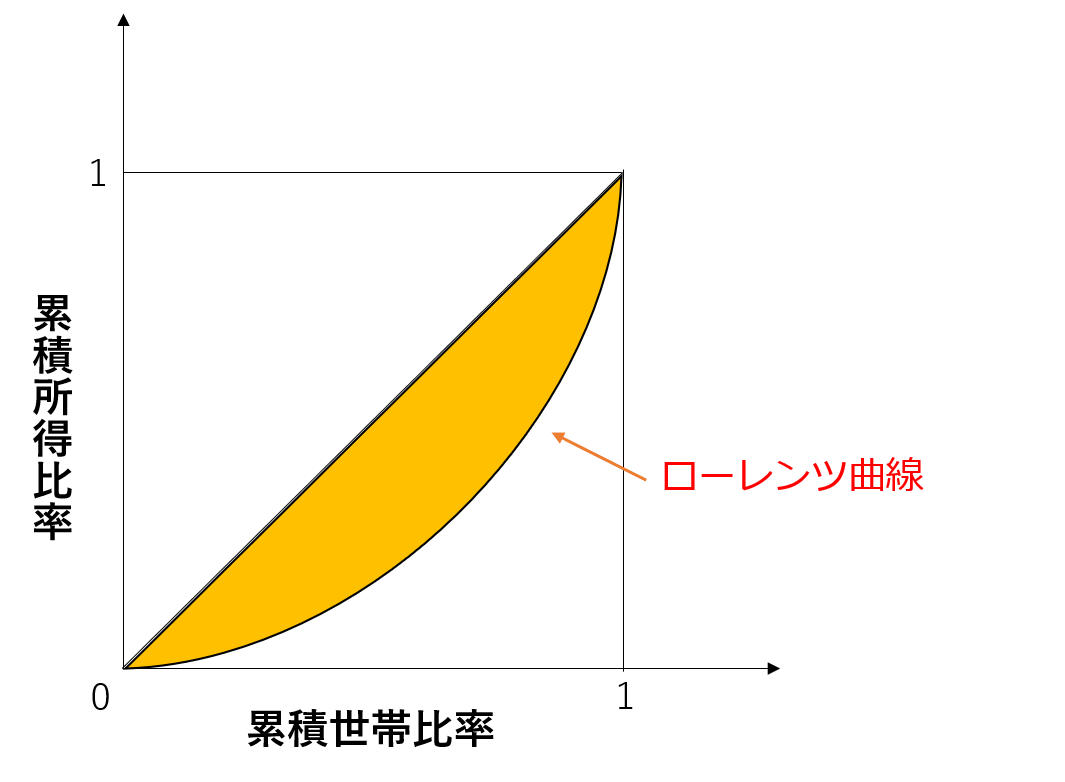
\includegraphics[width=7cm]{figure1}
\caption{ローレンツ曲線とジニ係数}
\end{figure}


\subsection{対数正規分布とジニ係数の関係}
この節では,定理\ref{t5}により対数正規分布のパラメータとジニ係数の関係を示す.その証明の準備として次の事実を示しておく.

\begin{thm}\label{t2}
対数正規分布$\Lambda(\mu_1, \sigma_1^2), \Lambda(\mu_2, \sigma_2^2)$に対し,次の式が成り立つ:
\begin{equation}
\int_0^{\infty} \Lambda(x\mid \mu_1, \sigma_1^2)\ d\Lambda(x\mid \mu_2, \sigma_2^2)
=\Lambda(1\mid \mu_1-\mu_2, \sigma_1^2+\sigma_2^2). \label{6}
\end{equation}
\end{thm}
\begin{proof}
$X,Y\geq 0$は独立で,$X\sim \Lambda(\mu_1, \sigma_1^2), Y\sim \Lambda(\mu_2, \sigma_2^2)$とし,$\dfrac{X}{Y}=Z$とする.
また,$X,Y,Z$の累積分布関数をそれぞれ$F(x),G(y),H(z)$とし,確率密度関数をそれぞれ$f(x),g(y),h(z)$とする.このとき,
\begin{align*}
H(1) &=\mathrm{Pr}\left( \frac{X}{Y}\leq 1\right) \\
&=\int_{\{\frac{X}{Y}\leq 1\}} f(x) g(y) \ dxdy \\
&=\int_0^{\infty} \int_0^1 f(yt) g(y) y \ dtdy \\
&=\int_0^{\infty} F(y)g(y) \ dy
\end{align*}
となる.

次に$H(z)$のパラメータについて確認する.
$X,Y$は対数正規分布に従っているので,$\log X\sim N(\mu_1, \sigma_1^2), \log Y\sim N(\mu_2, \sigma_2^2) $となる.
正規分布は再生性をもつため,
\[ \log \frac{X}{Y}=\log X-\log Y \sim N(\mu_1-\mu_2, \sigma_1^2+\sigma_2^2) \]
となる.よって,$Z\sim \Lambda(\mu_1-\mu_2, \sigma_1^2+\sigma_2^2)$となり,定理\ref{t2}が成り立つ.
\end{proof}

\begin{thm} \label{t5}
所得の分布が対数正規分布$\Lambda(\mu, \sigma^2)$に従い,ジニ係数がGとなるとき,次の式が成り立つ:
\begin{equation}
G=2N\left( \frac{\sigma}{\sqrt{2}}\relmiddle| 0,1\right) -1. \label{7}
\end{equation}
\end{thm}
\begin{proof}
所得の分布が対数正規分布$\Lambda(\mu, \sigma^2)$に従うとき,その累積分布関数を$\Lambda(x\mid \mu, \sigma^2)$とすると,累積世帯比率は$\Lambda(x\mid \mu, \sigma^2)$となる.よって,ローレンツ曲線の値を$F(x)$とすると,$\Lambda(\mu, \sigma^2)$の期待値$m$を用いて$F(x)$は次のように表せる:
\begin{align*}
F(x) &=\frac{1}{m}\int_0^x u\ d\Lambda(u\mid \mu, \sigma^2) \\
&=\exp \left( -\mu-\frac{\sigma^2}{2}\right) \int_0^x \exp (\log u)\frac{1}{\sqrt{2\pi}\sigma u}\exp \left\{ -\frac{1}{2\sigma^2}(\log u-\mu)^2\right\} du \\
&=\int_0^x \frac{1}{\sqrt{2\pi}\sigma u}\exp \left\{ -\frac{1}{2\sigma^2}(\log u-\mu-\sigma^2)^2\right\} du \\
&=\Lambda(x\mid \mu+\sigma^2,\sigma^2).
\end{align*}

したがって,所得の分布が$\Lambda(\mu, \sigma^2)$となるとき,ジニ係数を$G$とすると,
\begin{align*}
G &=1-2\int_0^{\infty}F(x)\ d\Lambda(x\mid \mu, \sigma^2) \\
&=1-2\int_0^{\infty}\Lambda(x\mid \mu+\sigma^2, \sigma^2)\ d\Lambda(x \mid \mu, \sigma^2) \\
&=1-2\Lambda(1\mid \sigma^2, 2\sigma^2) \hspace{1cm} \text{(\eqref{6}より)} \\
&=1-2N(0\mid \sigma^2, 2\sigma^2) \notag \\
&=1-2\left\{ 1-N\left( \frac{\sigma}{\sqrt{2}}\relmiddle| 0,1\right) \right\} \\
&=2N\left( \frac{\sigma}{\sqrt{2}}\relmiddle| 0,1\right) -1
\end{align*}
となる.
\end{proof}

%%%%%%%%%%%%%%%%%%%%%%%%%%%%%%%%%%%%%%%%%%%%%%%%%%%%%%%%%%%%%%%%%%%%%%%%%%%%%%%%%%%%%%%%%%%%%

\newpage
\section{ジニ係数の不偏推定}\label{suitei}
期待値が真の値に一致するような推定量を\textbf{不偏推定量}という.
本章ではサンプリングによってジニ係数の母数を推定する方法を与える.

\subsection{不偏推定量の予想}\label{yosou}
ジニ係数の不偏推定量がどのように表現できるか,計算機によるシミュレーションによって見当をつける.以下本論文ではRを用いてシミュレーションを行う.\eqref{5}より,$n$個の標本$y_1,y_2,\dotsb,y_n$からジニ係数を推定するとき,それらの母集団の平均$m$を用いて,以下の3式のいずれかで表せるのではないかと考えた:
\begin{align*}
G_1&=\frac{1}{2mn^2} \sum_{i=1}^n \sum_{j=1}^n |y_i-y_j| \\
G_2&=\frac{1}{2mn(n-1)} \sum_{i=1}^n \sum_{j=1}^n |y_i-y_j| \\
G_3&=\frac{1}{2m(n-1)^2} \sum_{i=1}^n \sum_{j=1}^n |y_i-y_j|. 
\end{align*}
$G_1,G_2,G_3$と母集団のジニ係数を比較する.
シミュレーションは以下のようにして行う.
\begin{enumerate}
\item ジニ係数が0.4となる母集団から10個の標本を採る.
\item 標本から$G_1,G_2,G_3$を求める.
\item この試行を10000回行い,その二乗平均平方根をとって比較する.
\end{enumerate}
シミュレーションを行った結果は以下のようになった.(Rのコードを付録\ref{app1}に記す.)
\begin{center}
$G_1$ : 0.3607858 \\
$G_2$ : 0.4008731 \\
$G_3$ : 0.4454146 \\
\end{center}
母集団のジニ係数が0.4となることからジニ係数の不偏推定量は$G_2$のように表現できるのではないかと予想した.


\subsection{予想した不偏推定量の証明}
本節では\ref{yosou}節で行った予想を定理としてまとめ,その証明を行う.
\begin{thm}
母集団が対数正規分布$\Lambda(\mu, \sigma^2)$に従っており,そこから$n$個の標本を採りジニ係数を推定する.ジニ係数の真の値を$G$とする.また,所得の標本の値を$x_1,x_2,\dotsb,x_n\ (n\geq 2)$,母集団の平均値を$m$($m$は既知の値)とする.このとき,$G$の推定値$\hat{G}$を,
\[ \hat{G}=\frac{1}{2mn(n-1)} \sum_{i=1}^n \sum_{j=1}^n |x_i-x_j| \]
とすると,
\[ E(\hat{G})=G \]
となる.
\end{thm}

\begin{proof}
$x_1,x_2,\dotsb,x_n$を並べ替えたものを$y_1\leq y_2\leq \dotsb \leq y_n$とすると,
\begin{align*}
\hat{G} &=\frac{1}{2mn(n-1)} \sum_{i=1}^n \sum_{j=1}^n |y_i-y_j| \\
&=\frac{2}{2mn(n-1)} \sum_{i=2}^n \sum_{j=1}^{i-1} (y_i-y_j) \\
&=\frac{1}{mn(n-1)} \sum_{i=1}^{n-1} (iy_{i+1}-\sum_{j=1}^i y_j) \\
&=\frac{1}{mn(n-1)} \sum_{k=1}^n (k-1)y_k -\frac{1}{mn(n-1)} \sum_{k=1}^n (n-k)y_k \\
&=\frac{1}{mn(n-1)} \sum_{k=1}^n (2k-n-1)y_k \\
&=\frac{1}{mn(n-1)} \sum_{k=1}^n 2ky_k-\frac{n+1}{mn(n-1)}mn \\
&=\frac{2}{mn(n-1)} \sum_{k=1}^n ky_k-\frac{n+1}{n-1}
\end{align*}
となる.よって,
\[ E(\hat{G})=\frac{2}{mn(n-1)} \sum_{k=1}^n kE(y_k)-\frac{n+1}{n-1} \]
となる.標本のうち$k$番目に大きいもの$Y_k$の確率密度関数を$f_r(y)$とすると,\eqref{9}より,
\begin{align*}
\sum_{k=1}^n kE(y_k) =&\sum_{k=1}^n k\int_0^{\infty} y k\binom{n}{k}F(y)^{k-1}\{1-F(y)\}^{n-k}f(y)\ dy \\
=&\int_0^{\infty} \sum_{k=1}^n kn\binom{n-1}{k-1}F(y)^{k-1}\{1-F(y)\}^{n-k}yf(y)\ dy \\
=&\int_0^{\infty} \sum_{k=1}^n \frac{(n-1)!}{(k-1)!(n-k)!} F(y)^{k-1}\{1-F(y)\}^{n-k}nyf(y)\ dy \\
 &+\int_0^{\infty} \sum_{k=1}^n (k-1)\frac{(n-1)!}{(k-1)!(n-k)!}F(y)^{k-1}\{1-F(y)\}^{n-k}nyf(y)\ dy \\
=&\int_0^{\infty} \{ F(y)+1-F(y)\}^{n-1}nyf(y)\ dy \\
 &+\int_0^{\infty} \sum_{k=2}^n (n-1)\frac{(n-2)!}{(k-2)!(n-k)!}F(y)^{k-2}\{1-F(y)\}^{n-k} F(y)nyf(y)\ dy \\
=&\int_0^{\infty} [1+(n-1)\{F(y)+1-F(y)\}^{n-2}F(y)]nyf(y)\ dy \\
=&\int_0^{\infty} \{1+(n-1)F(y)\} nyf(y)\ dy
\end{align*}
となるので,$E(\hat{G})$は
\begin{align*}
E(\hat{G}) &=\frac{2n}{mn(n-1)} \int_0^{\infty} \{1+(n-1)F(y)\}yf(y)\ dy-\frac{n+1}{n-1} \\
&=\frac{2}{m(n-1)} \int_0^{\infty} yf(y)\ dy+\frac{2}{m} \int_0^{\infty} F(y)yf(y)\ dy-\frac{n+1}{n-1} \\
&=\frac{2}{n-1} +\frac{2}{m} \int_0^{\infty} F(y)yf(y)\ dy-\frac{n+1}{n-1} \\
&=\frac{2}{m} \int_0^{\infty} F(y)yf(y)\ dy-1 \\
&=2\int_0^{\infty} \exp \left( -\mu-\frac{\sigma^2}{2} \right) F(y)y\frac{1}{\sqrt{2\pi}\sigma y}\exp \left\{ -\frac{(\log x-\mu)^2}{2\sigma^2} \right\} \ dy-1 \\
&=2\int_0^{\infty} F(y) \cdot \frac{1}{\sqrt{2\pi}\sigma y} \exp(\log y)\exp \left(-\mu-\frac{\sigma^2}{2} \right)\exp \left\{ -\frac{(\log x-\mu)^2}{2\sigma^2} \right\} \ dy-1 \\
&=2\int_0^{\infty} F(y) \cdot \frac{1}{\sqrt{2\pi}\sigma y} \exp \left\{ -\frac{(\log y-\mu-\sigma^2)^2}{2\sigma^2} \right\} \ dy-1 \\
&=2\int_0^{\infty} \Lambda(y\mid \mu, \sigma^2)\ d\Lambda(y\mid \mu+\sigma^2, \sigma^2)-1 \\
&=2\Lambda(1\mid -\sigma^2, 2\sigma^2)-1 \hspace{1cm} (\text{\eqref{6}より}) \\
&=2N(0\mid -\sigma^2,2\sigma^2)-1 \\
&=2N\left( \frac{\sigma}{\sqrt{2}}\relmiddle| 0,1\right) -1 \\
&=G \hspace{3cm} (\text{\eqref{7}より})
\end{align*}
となる.
\end{proof}
以下,ジニ係数の不偏推定量
\[ \hat{G}=\frac{1}{2mn(n-1)} \sum_{i=1}^n \sum_{j=1}^n |x_i-x_j| \]
を\textbf{不偏ジニ係数}と呼ぶ.

%%%%%%%%%%%%%%%%%%%%%%%%%%%%%%%%%%%%%%%%%%%%%%%%%%%%%%%%%%%%%%%%%%%%%%%%%%%%%%%%%%%%%%%%

\section{ジニ係数の比の検定} \label{kentei}
\subsection{ジニ係数の比の分布} \label{ginidist}
まず,ジニ係数の比と対数正規分布のパラメータ$\sigma$の比の関係について考える.
\eqref{7}より,
\begin{equation}
\sigma=\sqrt{2}N^{-1}\left( \frac{G+1}{2} \relmiddle| 0,1 \right) \label{10}
\end{equation}
が成り立ち,\eqref{10}をグラフに表すと図\ref{figure4}のようになる.

\begin{figure}[htbp]
\centering
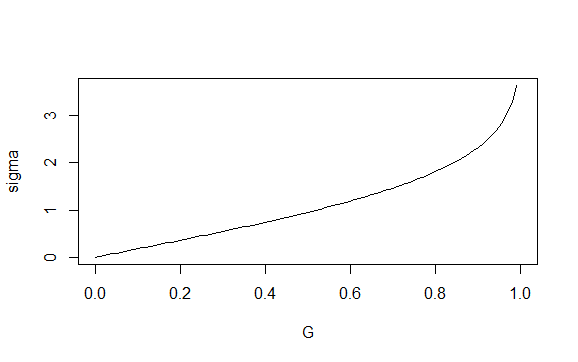
\includegraphics[width=8cm]{figure4}
\caption{}
\label{figure4}
\end{figure}

実際の国ごとのジニ係数$G$の値は$0.2<G<0.6$となる\cite{URL2}.図\ref{figure4}を見ると,この範囲で$G$と$\sigma$の関係は比例関係で近似できそうである.そこで,計算機によるシミュレーションを行い,
\[ \sigma=aG \]
と表したときに$0.2<G<0.6$の範囲で$\sigma$の誤差が最も小さくなるような$a$を見つける.

シミュレーションを行った結果,$a=1.935671$,そのときの$0.2<G<0.6$における$\sigma$の誤差の最大値は0.0288472となった.
(Rのコードを付録\ref{app2}に記す.)

したがって,ここでは$a=1.935671$として,
\begin{equation}
\sigma=aG \label{11}
\end{equation}
と近似させる.このとき,$\hat{G}$を\eqref{11}で変換したものを$\hat{\hat{\sigma}}$とすると,
\[ \hat{\hat{\sigma}}=a\hat{G} \]
となる.

また,ある2集団が正規分布に従っており,その母分散が$\sigma_1^2$,$\sigma_2^2$のとき,サンプル数を共に$n$,不偏分散をそれぞれ$\hat{\sigma_1^2}$,$\hat{\sigma_2^2}$とすると,定理\ref{t3}より,
\[ \frac{\hat{\sigma_1^2}/\sigma_1^2}{\hat{\sigma_2^2}/\sigma_2^2} \sim F(n-1,n-1) \]
となる.

不偏ジニ係数から導いた値$\hat{\hat{\sigma}}^2$と不偏分散$\hat{\sigma^2}$は近い値になるのではないかと考え,
\[ \frac{\hat{G_1}^2/G_1^2}{\hat{G_2}/G_2^2} = \frac{\hat{\hat{\sigma_1}}^2/\sigma_1^2}{\hat{\hat{\sigma_2}}^2/\sigma_2^2}  \sim F(\phi, \phi) \]
となるのではないかと考えた.そこで,$F$分布に従っているとしたとき,そのパラメータすなわち自由度$\phi$がどのようになるのかを計算機によるシミュレーションによって求める.シミュレーションを行った結果は以下のようになった.(Rのコードを付録\ref{app3}に記す.)
\vspace{2mm}

\scalebox{0.8}{
\begin{tabular}{|c||c|c|c|c|c|c|c|c|c|} \hline
 & 0.3/0.3 & 0.3/0.4 & 0.3/0.5 & 0.4/0.3 & 0.4/0.4 & 0.4/0.5 & 0.5/0.3 & 0.5/0.4 & 0.5/0.5 \\ \hline \hline
10 & 9.0628 & 8.55491 & 9.79464 & 9.06198 & 9.15999 & 9.78654 & 9.50342 & 9.77336 & 9.65049 \\ \hline
20 & 18.24722 & 18.17889 & 17.82843 & 18.65292 & 18.54466 & 18.61361 & 16.23197 & 18.64238 & 19.00748 \\ \hline
30 & 27.43193 & 27.39329 & 25.91775 & 26.93673 & 26.52706 & 27.18588 & 27.68051 & 27.30638 & 28.47172 \\ \hline
40 & 37.772 & 35.99459 & 36.35678 & 35.123 & 36.26493 & 36.58253 & 32.94116 & 35.53869 & 34.74861 \\ \hline
50 & 45.63523 & 43.93531 & 44.89669 & 44.67966 & 44.81807 & 44.21327 & 45.72323 & 41.36189 & 43.90748 \\ \hline
60 & 54.69146 & 56.30184 & 52.54006 & 49.58406 & 53.28106 & 52.25395 & 53.28227 & 53.38646 & 51.80857 \\ \hline
70 & 63.43626 & 62.97759 & 63.5802 & 59.44177 & 61.99081 & 59.97619 & 61.40957 & 59.89812 & 59.68023 \\ \hline
80 & 68.59902 & 73.24108 & 70.69003 & 69.27793 & 67.27696 & 68.49169 & 71.19527 & 68.52169 & 65.82451 \\ \hline
90 & 81.45638 & 77.198 & 76.89074 & 79.47248 & 75.29302 & 77.69753 & 76.22371 & 74.80826 & 73.96592 \\ \hline
100 & 87.76654 & 90.81742 & 87.37898 & 85.71286 & 89.90437 & 89.663 & 89.26296 & 82.28468 & 86.21494 \\ \hline
\end{tabular}
}
\\\ 

上の表はサンプル数を10から100まで,2つの母集団のジニ係数($G_1/G_2$)を0.3から0.5まで変化させたとき,$\dfrac{\hat{G_1}^2/G_1^2}{\hat{G_2}^2/G_2^2}$の分布と累積分布関数間の差の絶対値の最大値が最も小さくなるような$F$分布の自由度を表示したものである.
この結果から,$\dfrac{\hat{G_1}^2/G_1^2}{\hat{G_2}^2/G_2^2}$が従う$F$分布の自由度$\phi$を
\[ \phi=n-\frac{n-10}{10} \]
として再びシミュレーションによって累積分布関数の誤差を求めると下の表のようになった.(Rのコードを付録\ref{app4}に記す.)
\vspace{2mm}

\scalebox{0.8}{
\begin{tabular}{|c||c|c|c|c|c|c|c|c|c|} \hline
 & 0.3/0.3 & 0.3/0.4 & 0.3/0.5 & 0.4/0.3 & 0.4/0.4 & 0.4/0.5 & 0.5/0.3 & 0.5/0.4 & 0.5/0.5 \\ \hline \hline
10 & 0.02119 & 0.0241 & 0.03115 & 0.02607 & 0.0145 & 0.0318 & 0.03513 & 0.02582 & 0.00568 \\ \hline
20 & 0.01173 & 0.02246 & 0.03357 & 0.01277 & 0.01243 & 0.02089 & 0.03424 & 0.02036 & 0.006 \\ \hline
30 & 0.01484 & 0.01278 & 0.0364 & 0.0124 & 0.01098 & 0.01994 & 0.03673 & 0.02301 & 0.00949 \\ \hline
40 & 0.00715 & 0.01137 & 0.02945 & 0.01117 & 0.01154 & 0.03383 & 0.02551 & 0.02552 & 0.01258 \\ \hline
50 & 0.00667 & 0.01704 & 0.02886 & 0.01816 & 0.00589 & 0.02664 & 0.03327 & 0.02489 & 0.01098 \\ \hline
60 & 0.01033 & 0.00902 & 0.02362 & 0.01882 & 0.00792 & 0.02126 & 0.02391 & 0.01782 & 0.00831 \\ \hline
70 & 0.01097 & 0.01479 & 0.02673 & 0.00672 & 0.01031 & 0.02122 & 0.02186 & 0.01908 & 0.01552 \\ \hline
80 & 0.00822 & 0.02315 & 0.02334 & 0.01665 & 0.00775 & 0.01487 & 0.02046 & 0.01708 & 0.01305 \\ \hline
90 & 0.01038 & 0.01724 & 0.02861 & 0.01293 & 0.00718 & 0.02057 & 0.02236 & 0.01671 & 0.01589 \\ \hline
100 & 0.0058 & 0.01084 & 0.01304 & 0.01293 & 0.01538 & 0.02261 & 0.03094 & 0.01121 & 0.01583 \\ \hline
\end{tabular}
}
\\\ 

表を見ると累積分布関数間の誤差が0.03程度に収まっていることが分かる.実際,$n=10,G_1=G_2=0.4$のときの$\dfrac{\hat{G_1}^2/G_1^2}{\hat{G_2}^2/G_2^2}$の分布と$F(\phi, \phi)$($\phi=n-\dfrac{n-10}{10}$)の確率密度関数は図\ref{figure10}のようになり,F分布で近似できていることが分かる.
\begin{figure}[htbp]
\centering
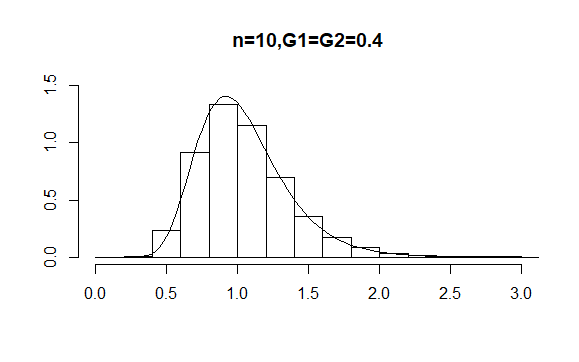
\includegraphics[width=8cm]{figure10}
\caption{}
\label{figure10}
\end{figure}
以上より,ジニ係数が$G_1$,$G_2$となる2集団から導いた不偏ジニ係数を$\hat{G_1}$,$\hat{G_2}$,サンプル数を共に$n$としたとき,
\[ \frac{\hat{G_1}^2/G_1^2}{\hat{G_2}^2/G_2^2} \sim F(\phi, \phi) \]
とする.このとき$\phi$は,
\[ \phi=n-\frac{n-10}{10} \]
である.


\subsection{検定手順}
$F$検定の手法を参考にしてジニ係数の比の検定を行う.ここでは,サンプルサイズの設計を見越して,2集団から採るサンプルの数は等しいものと考える.
\begin{enumerate}[label=手順\arabic*]
\item 仮説の設定\\
2つの集団のジニ係数をそれぞれ$G_1$,$G_2$($G_1\geq G_2$)とする.
このとき,帰無仮説と対立仮説を次のように設定する:\\
帰無仮説 $ H_0 : G_1=G_2$ \\
対立仮説 $ H_1 : G_1>G_2$.
\item 有意水準$\alpha$の設定 ($\alpha =0.05$とする)
\item 棄却域$R$の設定
\[ R : F_0\geq F(\phi, \phi; \alpha) \]
このとき,
\[ \phi=n-\frac{n-10}{10} \]
\item データ $ x_{11}, x_{12}, \dotsb, x_{1n} $ および $ x_{21}, x_{22}, \dotsb, x_{2n} $ をとり,検定統計量$F_0$の値を計算する.
ここで,$m$は母集団の平均値で既知の値である.
\begin{align*}
F_0 &=\frac{G_1^2}{G_2^2} \\
G_1 &=\frac{1}{2mn(n-1)} \sum_{i=1}^n \sum_{j=1}^n |x_{1i}-x_{1j}| \\
G_2 &=\frac{1}{2mn(n-1)} \sum_{i=1}^n \sum_{j=1}^n |x_{2i}-x_{2j}|
\end{align*}
\item $F_0$が手順3で設定した棄却域$R$にあれば有意と判定し,$H_0$を棄却する.
\end{enumerate}


\subsection{検出力の導出とサンプルサイズの設計} \label{ex}
\ref{ftest}節を参考にすると検出力$1-\beta$は,
\[ 1-\beta = \mathrm{Pr} \left\{ F\geq \frac{F(\phi, \phi; \alpha)}{\Delta^2} \right\} \]
となる.ここで,
\[ \phi=n-\frac{n-10}{10}, \hspace{3mm} \Delta=\frac{G_1}{G_2} \hspace{2mm} \text{($G_1,G_2$は$H_1$におけるもの)} \]
である.

$\Delta \geq \Delta_0$のとき高い検出力$1-\beta$で$H_0$を棄却したい.
\ref{ftest}節を参考にすると,
\[ \phi \approx \left( \frac{z_{\alpha}-z_{1-\beta}}{\log \Delta_0} \right)^2 \]
が成り立つ.$ \phi=n-\dfrac{n-10}{10} $を上式に代入して式を整理すると,サンプルサイズ$n$は,
\begin{equation}
n \approx \frac{10}{9} \left\{ \left( \frac{z_{\alpha}-z_{1-\beta}}{\log \Delta_0} \right)^2-1 \right\} \label{12}
\end{equation}
となる.

サンプルサイズの設計の例を考える.
集団Aと集団Bのジニ係数をそれぞれ$G_1,G_2 \hspace{1mm} (G_1 \geq G_2)$とする.このとき,帰無仮説$H_0$を$G_1=G_2$,対立仮説$H_1$を$G_1>G_2$,有意水準$\alpha$を$\alpha=0.05$とする.$\Delta=\dfrac{G_1}{G_2} \geq \Delta_0$のとき,検出力$1-\beta=0.8$で$H_0$を棄却したい.\eqref{12}より,必要なサンプルサイズ$n$は次のようになる.
\begin{equation}
n \approx \frac{10}{9} \left\{ \left( \frac{z_{0.05}-z_{0.8}}{\log \Delta_0} \right)^2-1 \right\} \label{13}
\end{equation}
\eqref{13}をグラフに表すと図\ref{sizecurve}のようになる.
\begin{figure}[htbp]
\centering
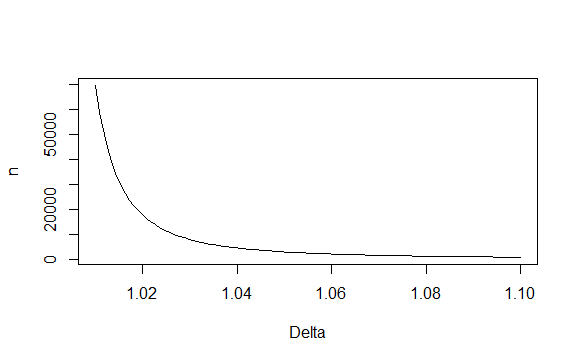
\includegraphics[width=8cm]{figure5}
\caption{}
\label{sizecurve}
\end{figure}

\eqref{13}は,母集団のジニ係数の比が$\Delta_0$以上のとき検出力を0.8とするためには標本は$n$人採れば十分だということを意味している.
実際の世界各国のジニ係数は表1のようになるため,対立仮説のジニ係数の比が1.1以上となることは多いと考えられる.\eqref{13}において$\Delta_0=1.1$のとき$n=755.107$となる.
世界のほとんどの国の人口は756人よりずっと多いため,これは有意義な結果であったと言える.また,市区町村のような集団であってもこの規模の標本を採ることは可能なので,国家のような大きな集団で無くとも今回提案したジニ係数の比の検定は意味を持つと考えられる.

%%%%%%%%%%%%%%%%%%%%%%%%%%%%%%%%%%%%%%%%%%%%%%%%%%%%%%%%%%%%%%%%%%%%%%%%%%%%%%%%%%%%%%%%%%%%%%%%%%

\section{考察・まとめ}
本論文では大きく2つのことを行った.1つは不偏ジニ係数の発見及び証明,もう1つはジニ係数の比の検定方法の提案である.

不偏ジニ係数の不偏性の証明は手探りの状態で計算を進めていたため,順序統計量をうまく利用して証明することができてよかった.
ただし,不偏ジニ係数の式中に出てくる対数正規分布の平均$m$は既知の値である.これを使わずに不偏推定量を表すことが今後の課題である.

ジニ係数の比の検定方法の提案では,検定の際に検出力をある程度まで高めるために必要なサンプル数を求めることができた.しかし,\ref{ginidist}節で示したようにジニ係数の比の分布と$F$分布の間には誤差が存在するため,サンプル数の式にも誤差が生じる.その誤差がどの程度のものなのかを明確に示すこと,あるいは,ジニ係数の比の分布を$F$分布とは別の分布で正確に表すことが今後の課題である.

%%%%%%%%%%%%%%%%%%%%%%%%%%%%%%%%%%%%%%%%%%%%%%%%%%%%%%%%%%%%%%%%%%%%%%%%%%%%%%%%%%%%%%%%%%%%%%%%%%

\section*{謝辞}
本論文を作成するにあたり,ご指導を頂きました指導教員の宮部賢志先生に深く感謝致します.宮部先生には,不偏性の証明を進める際やジニ係数の分布を考える際など,研究を進めるにあたって数多くのご助言を頂きました.また,論文の執筆にあたってもその書き方などを細かく指導して頂きました.ここに心から感謝致します.


\begin{thebibliography}{99}
\bibitem{stat} 稲垣宣生,『数理統計学(改訂版)』,裳華房,2003
\bibitem{R} 奥村晴彦,『Rで楽しむ統計』,共立出版,2016
\bibitem{geho} 下方拓,「格差分布の統計的ダイナミクス」,世界平和研究所,2008
\bibitem{size} 永田靖,『サンプルサイズの決め方』,朝倉書店,2003
\bibitem{yosida} 吉田建夫,「世界的所得分配の計測:1962-2000年」,『岡山大学経済学会雑誌』46,2014
\bibitem{URL1} ”国民生活基礎調査の概要|厚生労働省”,\url{<http://www.mhlw.go.jp/toukei/saikin/hw/k-tyosa/k-tyosa16/index.html>},2017年1月20日アクセス
\bibitem{URL2} ”世界のジニ係数 国別ランキング・推移”,\url{<https://www.globalnote.jp/post-12038.html>},2017年1月20日アクセス
\end{thebibliography}


\newpage
\appendix
\section{プログラムのコード}
\subsection{ジニ係数の不偏推定量} \label{app1}
\begin{lstlisting}
#サンプル数
n <- 10

#試行回数
N <- 10000

#母集団のジニ係数
g <- 0.4

#母集団の平均所得
m <- 550

#分布のパラメータを導く
sigma <- sqrt(2)*qnorm((g+1)/2)
mu <- log(m)-sigma^2/2

#ジニ係数を求める試行の繰り返し
g1 <- numeric(N)
g2 <- numeric(N)
g3 <- numeric(N)
for(i in 1:N){
  r <- rlnorm(n,mean=mu,sd=sigma)
  mr <- mean(r)
  a <- matrix(0,n,n)
  for(j in 1:n){
    for(k in 1:n){
      a[j,k] <- abs(r[j]-r[k])
    }
  }
  d <- sum(a)
  g1[i] <- (d/n^2)/(2*mr)
  g2[i] <- (d/(n*(n-1)))/(2*mr)
  g3[i] <- (d/(n-1)^2)/(2*mr)
}

#二乗平均平方根を表示する
print(sqrt(mean(g1^2)))
print(sqrt(mean(g2^2)))
print(sqrt(mean(g3^2)))
\end{lstlisting}



\subsection{$G$と$\sigma$の関係} \label{app2}
\begin{lstlisting}
#ジニ係数の範囲
G <- c(0.2,0.6)

#G-sigmaの関係式
sigma <- sqrt(2)*qnorm((G+1)/2)

#Gの定数倍で近似させたときの誤差の最大値
f <- function(s){
  max(abs(sigma-s*G))
}

#誤差の最大値を最も小さくするような定数
p <- optimize(f,c(1,3))
print(p)
\end{lstlisting}



\subsection{$F$分布の自由度} \label{app3}
\begin{lstlisting}
#試行回数
N <- 10000

#不偏ジニ係数
fg1 <- numeric(N)
fg2 <- numeric(N)

#母集団の平均所得
mu <- 100

#結果を表示させる表を作る
mat <- matrix(0,nrow=10,ncol=9)
df <- data.frame(mat)
#サンプル数
rn <- seq(10,100,by=10)
#母集団のジニ係数
rg <- seq(0.3,0.5,by=0.1)
colname <- c("0.3/0.3","0.3/0.4","0.3/0.5","0.4/0.3","0.4/0.4","0.4/0.5",
             "0.5/0.3","0.5/0.4","0.5/0.5")
rownames(df) <- rn
colnames(df) <- colname

for(n in rn){
  for(g1 in rg){
    for(g2 in rg){
      sigma1 <- sqrt(2)*qnorm((g1+1)/2)
      sigma2 <- sqrt(2)*qnorm((g2+1)/2)

   #不偏ジニ係数を求める繰り返し
      for(i in 1:N){
        r <- rlnorm(n,mean=mu,sd=sigma1)
        mr <- mean(r)        
        a <- matrix(1:n^2,n,n)
        for(j in 1:n){
          for(k in 1:n){
            a[j,k] <- abs(r[j]-r[k])
          }
        }
        d <- sum(a)
        fg1[i] <- (d/(n*(n-1)))/(2*mr)
      }      
      for(i in 1:N){
        r <- rlnorm(n,mean=mu,sd=sigma2)
        mr <- mean(r)
        a <- matrix(1:n^2,n,n)
        for(j in 1:n){
          for(k in 1:n){
            a[j,k] <- abs(r[j]-r[k])
          }
        }
        d <- sum(a)
        fg2[i] <- (d/(n*(n-1)))/(2*mr)
      }

      #ジニ係数の比の分布と分布関数間の誤差が最も小さくなるようなF分布の自由度を求める
      rate <- ((fg1/g1)/(fg2/g2))^2
      dfrate <- ecdf(rate)
      f <- function(s){
        max(abs(dfrate(rate)-pf(rate,s,s)))
      }
      p <- optimize(f,c(0,n+50))

      #求めた自由度を表に入力する
      if(g1==0.3){
        df[n/10,g2*10-2] <- round(p$minimum,5)
      }else{
        if(g1==0.4){
          df[n/10,g2*10+1] <- round(p$minimum,5)
        }else{
          df[n/10,g2*10+4] <- round(p$minimum,5)
        }
      }
    }
  }
}
\end{lstlisting}


\subsection{$F$分布との誤差} \label{app4}
\begin{lstlisting}
#試行回数
N <- 10000

#不偏ジニ係数
fg1 <- numeric(N)
fg2 <- numeric(N)

#母集団の平均所得
mu <- 100

#結果を表示させる表を作る
mat <- matrix(0,nrow=10,ncol=9)
df <- data.frame(mat)
#サンプル数
rn <- seq(10,100,by=10)
#母集団のジニ係数
rg <- seq(0.3,0.5,by=0.1)
colname <- c("0.3/0.3","0.3/0.4","0.3/0.5","0.4/0.3","0.4/0.4","0.4/0.5",
             "0.5/0.3","0.5/0.4","0.5/0.5")
rownames(df) <- rn
colnames(df) <- colname

for(n in rn){
  for(g1 in rg){
    for(g2 in rg){
      sigma1 <- sqrt(2)*qnorm((g1+1)/2)
      sigma2 <- sqrt(2)*qnorm((g2+1)/2)

   #不偏ジニ係数を求める繰り返し
      for(i in 1:N){
        r <- rlnorm(n,mean=mu,sd=sigma1)
        mr <- mean(r)       
        a <- matrix(1:n^2,n,n)
        for(j in 1:n){
          for(k in 1:n){
            a[j,k] <- abs(r[j]-r[k])
          }
        }
        d <- sum(a)
        fg1[i] <- (d/(n*(n-1)))/(2*mr)
      }      
      for(i in 1:N){
        r <- rlnorm(n,mean=mu,sd=sigma2)
        mr <- mean(r)        
        a <- matrix(1:n^2,n,n)
        for(j in 1:n){
          for(k in 1:n){
            a[j,k] <- abs(r[j]-r[k])
          }
        }
        d <- sum(a)
        fg2[i] <- (d/(n*(n-1)))/(2*mr)
      }

      #ジニ係数の比の分布と設定した自由度のF分布との分布関数間の誤差の最大値
      rate <- ((fg1/g1)/(fg2/g2))^2
      dfrate <- ecdf(rate)
      error <- round(max(abs(dfrate(rate)-pf(rate,n-(n-10)/10,n-(n-10)/10))),5)

      #求めた誤差を表に入力する
      if(g1==0.3){
        df[n/10,g2*10-2] <- error
      }else{
        if(g1==0.4){
          df[n/10,g2*10+1] <- error
        }else{
          df[n/10,g2*10+4] <- error
        }
      }
    }
  }
}
\end{lstlisting}


\end{document}

